\chapter{Introduction} 
This introduction contains the project goals and some very short introductions on the FPGAs and how they are used, numerical methods for approximating ODEs, functional programming and \clash{}. The short introductions are included for the sake of completeness and are assumed knowledge for the rest of the thesis.

\section{Project goals}
From the start, this project has had two main goals: firstly, obtaining information on the feasibility and the advantages and disadvantages of performing numerical mathematics (numerical approximations to ODEs) directly on (programmable) hardware, the FPGA. Secondly: figuring out whether higher-order functions are of much use for numerical mathematics. As per usual, having main goals spawns off several minor goals which support the main parts. Both supporting goals are about simplifying the process of configuring FPGAs: an easy way of setting up projects with complicated IO requirements and furthermore, developing a tool-chain integration which turns the long process of compiling and deploying your FPGA project into the execution of a single command.

Alongside these concrete goals the underlying theme is to do as much work as possible in \clash{}, a library and compiler based on the functional programming language Haskell, developed by Christiaan Baaij at the CAES group at the University of Twente. Further elaboration on \clash{} can be found in section \ref{s:clash}.


\section{FPGAs}
\subsection{What is an FPGA?}
An FPGA (Field Programmable Gate Array) is a chip in which you can specify the hardware yourself. In contrast to regular programming in which you generate a long list of instructions which are executed sequentially on a fixed chip configuration, the FPGA allows you to specify exactly which wire (signal) leads where and what operation should be applied to that signal. This approach to programming can have several advantages. The first one arises from the large opportunities for parallelism. Every part of the FPGA can be executing a meaningful computation simultaneously, whereas processors are bound by the amount of physical cores they have in the amount of truly concurrent instruction executions possible. Secondly, a conventional processor only has a fixed instruction set. Using an FPGA you can define your own instructions (subcircuits), again providing a possible improvement in computational speed. According to \cite{FPGAvsCPU}, FPGAs were already capable of outperforming CPUs on very parallelizable numerical tasks on single and double precision floating point numbers in as early as 2004. Furthermore, as you are implementing your signal processing directly in hardware, there will be a fixed bound on the possible latency. This makes FPGAs ideal for purposes in high-throughput, low-latency signal processing, eg. real-time audio, video or data stream processing. Lastly, the reconfigurability of FPGAs whilst remaining close to the actual hardware allows for cost reductions in the verification of ASIC (Application-Specific Integrated Circuits) designs. It's cheaper to reprogram your FPGA than to have a new version of an ASIC manufactured.

However, the FPGA is a trade-off between implementing designs directly in hardware and being able to run multiple designs (after a reconfiguration). As a consequence of this, it still loses to ASICs with several orders of magnitude on performance \cite{FPGAvsASIC} and CPUs still dominate in terms of versatility and on-the-fly reconfigurability.

\subsection{How does it work?}
An FPGA is built up from several distinct element types, depicted in figure \ref{f:fpga_fabric}
\begin{enumeratens}
	\item \emph{Logic elements} Responsible for the actual signal processing. An FPGA may contain different types of logic elements, eg. memory, DSP and logic blocks. These blocks implement some signal processing capability which can be configured up to certain limits.
	\item \emph{Programmable interconnects} In order to be able to represent complex designs, the logic elements need to be connected in a certain way. This is what the programmable interconnects are for. Essentially, those are wires which can be turned on and off by the user as part of a design specification. 
	\item \emph{IO blocks} Finally, the functionality implemented using the logic elements and programmable interconnects should be exposed to external signals in order to be useful. IO blocks can be used to control hardware pins, controlling a LED or reading a switch but also for more intricate IO facilities, eg. external memory controllers.
\end{enumeratens}

\begin{figure}[h]
	\centering
	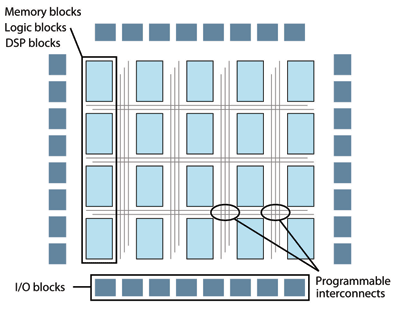
\includegraphics[width=0.45\textwidth]{fpga_fabric}
	\caption{FPGA fabric.}
	\label{f:fpga_fabric}
\end{figure}

It might seem that programming an FPGA involves manually specifying the interconnects and exact configurations of the logic elements. However, specialized languages have been developed just for the purpose of describing the FPGA functionality at a higher level of abstraction and leave the specific routing and assignment of logic elements to the compiler. The two main advantages of these languages are that you do not have to worry about low-level problems like how the interconnects will be routed and secondly, your written specification will be portable across multiple FPGA vendors as long as the vendor supplies you with the proper compiler from your specification to a file which can be used to program the FPGA. 

More information on FPGA functionality can be found in \cite{FPGAexplained}.


\subsection{System-on-a-chip}
FPGAs in itself can be useful, but especially for design with IO requirements that are more complex than just reading out hardware switches and controlling LEDs, more control is needed. This requirement has led to the rise of SoCs (System-on-Chip). These devices integrate an FPGA with additional hardware on a single chip. This extra hardware usually contains a CPU, which can be used to simplify the process of loading and extracting data from the FPGA. The SoC used for this thesis is the Terasic SoCKit, a development kit containing an Altera Cyclone V FPGA and a dual-core ARM A9 CPU on a single chip (Altera 5CSXFC6D6F31C6N), alongside a wide variety of IO possibilities. Further information on the SoC used is available at \cite{SoCKit}.

\section{Numerical solvers for ODEs}
The field of numerical solvers is a vast and active area of research. Furthermore, there is a lot of theory on which solver to pick for specific problems, related to stability, computational efficiency and other factors. However, the goal of this thesis is to get an impression of the feasibility of using numerical solvers for ODEs on FPGAs. Therefore, the selection of solvers will be restricted to some very basic schemes. 

The solvers used have some common properties:
\begin{itemizens}
	\item \emph{Fixed-step} The solvers compute a value for the ODE at a fixed step size. This means that in contrary to the continous 'mathematical' solution of an ODE, the output of the solver will be an approximate to the actual value of the solution at the discrete set of values of the independent variable, in which the difference between the values of the independent variables is defined by the fixed step size.
	\item \emph{Single-step} The approximate value of the ODE $x_{k}$ at $t_{k}$ only depends on $t_{k-1}$, $x_{k-1}$ and the ODE that is being approximated.   
\end{itemizens}

\subsubsection{Euler}
The easiest numerical solver, without doubt, is Euler's method (equation \ref{eq:euler}). For every discrete point in time, the value of the next point is approximately equal to the derivative at that point multiplied by the time step added to the current value. The simplicity of the scheme has a cost: it is not very accurate and the errors accumulate quickly. From \cite{DE}, the maximum error of Euler's method can be shown to be linear in the time step and exponential in the interval length (eq \ref{eq:euler_error}), in which $M$ and $L$ are constants depending on the equation to be solved, $b-a$ is the solution interval length and $h$ is the time step.

\begin{align}
	\label{eq:euler}
	s_{k,1} &= f(t_{k},x_{k}) \\
	x_{k+1} &= x_{k} + h s_{k,1} \nonumber
\end{align}

\begin{equation}
\label{eq:euler_error}
\text{maximum error}_{\text{euler}} \leq \frac{M h}{L} (e^{L(b-a)} -1)
\end{equation}

\subsubsection{Runge-Kutta methods}
The Runge-Kutta methods are a family of solvers, of which the 4th order version is the most well-known (RK4). The solver used here will be a second-order Runge-Kutta method, also known as the \emph{improved Euler's method} \cite{DE}. This second order method requires the computation of two slopes (equation \ref{eq:rk2}), in contrast to the single one required for Euler's method.

\begin{align}
	\label{eq:rk2}
	s_{k,1} &= f(t_{k},x_{k}) \\
	s_{k,2} &= f(t_{k} + h,x_{k} + h s_{k,1}) \nonumber \\
	x_{k+1} &= x_{k} + h \frac{s_{k,1} + s_{k,2}}{2} \nonumber
\end{align}

\begin{equation}
\label{eq:rk2_error}
\text{maximum error}_{\text{RK2}} \leq \frac{M h^{2}}{L} (e^{L(b-a)} -1)
\end{equation}

Note that the maximum error of RK2 is proportional to the square of the time step (equation \ref{eq:rk2_error}). As the time step decreases by a factor of 2, the maximum error will decrease by a factor of 4, given that the equation and the range stay the same. However, the maximum error still depends exponentially on the interval length.


\section{Functional programming}
\subsection{What is functional programming?}
The three most important concepts are:
\subsubsection{Expressions}
\subsubsection{Functions}
\subsubsection{Referential transparency}
\subsubsection{Referential transparency}

\cite{FPIntro}
\subsection{Using FP for numerical mathematics}
Functional languages have several properties which make them suitable for the purpose of solving problems in numerical mathematics. First and foremost, Haskell, being based on $\lambda$-calculus is very close to mathematics. The useful mathematical properties here are \textit{referential transparency}, easy \textit{partial function application} and being a \textit{declarative language}. 
Referential transparency implies that a variable only has a constant value which is the same everywhere in the program. This prevents that changing a variable might have influence on another computation as a side effect and it corresponds to mathematical notation. For instance, in an imperative programming like C you could write \code{i = i + 1}, which is a mathematical impossibility and therefore not allowed in Haskell. 
Partial function application is another very useful concept. Often in numerical mathematics, you want to create or process a function. You need a function that has another function as return value. For instance, take a function which requires two arguments. After only applying a single argument, the object returned still needs the second argument in order to compute the final value. This is exactly according to the definition of a function: An object that still needs arguments before being able to return its final value.
Being a \textit{declarative language} means that you write code that specifies what you want to accomplish, not how to get there. This concept is again borrowed from mathematics. You put in a set of function definitions and Haskell will figure out how to actually compute the value you request according to those definitions. This property of declarativity also has the result that Haskell is a terse language whilst remaining easy to understand.
Secondly, Haskell has a very strong type system. The type system has three main advantages. It becomes very easy to swap out and replace functions as long as you make sure that the types are the same. The Haskell compiler will start to assert errors immediately whenever you feed it something which does not make sense or could be ambiguous which is very useful when writing programs. By having a look at the types of a Haskell program it becomes very straightforward to see what the program does and how it works, which is very useful when attempting to understand your own or someone else's code.
Lastly, a property which is often very important for numerical mathematics: Haskell is fast. According to the \textit{Computer Language Benchmarks Game} \cite{Bench}, Haskell is almost on par with Java and Fortran but significantly faster than Python and Matlab (not shown), two languages which are often used for numerical mathematics nowadays. There is still a performance gap of around a factor 3 between Haskell and C (the reference), hence if speed is of the absolute highest concern C is still a valid option.

\subsection{Example: Numerical solutions of ODEs in Haskell}

\lstset{style=haskellStyle}

As mentioned before, the types in Haskell reveal lots of information about the structure and functionality of the program. The three main types constituting the numerical solver for ordinary differential equations are listed above.

\lstinputlisting[caption=Main types for the ODE solver, label=solvertypes, firstline=18]{../haskell/SolverTypes.hs}

\subsubsection{Equation}
In essence, a differential equation is a mapping (function) from a certain state of the system to the change of this system. This is also what the type signature of \code{Equation} signifies, a mapping from an \code{ODEState} to a \code{D_ODEState}. This generic set up allows the specification of any ODE for solving. The implementation in pure Haskell of a simple ODE is given in listing \ref{lst:eq_exponential}, which corresponds to the equation $x' = -x$. However, this representation is not very elegant and a lot of the code is performing unboxing of the types. Using property that this equation is linear, it is possible to use an utility method which takes as input a matrix and returns the Haskell differential equation function belonging to that matrix. The same can be done for heterogeneous linear systems using a different utility function, which does not only takes a matrix as input but also a list of functions representing the heterogeneous part of the equation. The example code for this can be seen in appendix \ref{app:haskellsolver}.

\lstinputlisting[caption=Example equation for exponential decay, label=lst:eq_exponential, firstline=11,lastline=14]{../haskell/SolverEquations.hs}

\subsubsection{SolveMethod}
The \code{SolveMethod} performs the actual computations on what the next value of the solution should be: the integration scheme. In order to obtain this next state, the scheme needs three input values: It needs information on the timing constraints of the solution, in this case it needs the time step. Furthermore, it needs the equation itself and it requires the state of the system at $t_{n}$ in order to be able to determine the state of the system at $t_{n+1} = t_{n} + \Delta t$.

The most straightforward integration scheme is called forward Euler, given in equation \ref{eq:euler}. Listing \ref{lst:euler} depicts the translation of the mathematical expression \ref{eq:euler} to Haskell. Even though some list operations have been inserted (\code{zipWith} and \code{map}), the structure is still recognizable. It computes the change in state, multiplies this with the time step obtained in line 6 and adds the initial state in line 4. Lastly, the integration scheme returns the new state of the equation, consisting of a list of x-values and a corresponding time value. Implementations of different solvers (eg. 4th order Runge-Kutta) can be found in appendix \ref{app:haskellsolver}.

\lstinputlisting[caption=Example code for the Euler integration scheme, label=lst:forward_euler, firstline=9,lastline=15]{../haskell/SolverSolvers.hs}

\subsubsection{Solver}
The \code{Solver} function in listing \ref{lst:solver_frame} acts as the main interface to the program. You specify a \code{SolveMethod}, the \code{TimeSettings} (containing the time step and the time at which to stop solving), the equation itself and an initial condition. The \code{Solver} will then return a list of states of the system. As is very common in functional programming, the \code{Solver} has been defined recursively. Line 4 is where the magic happens: the solution list is defined to be the initial condition, followed by the solution list with the new state (computed by the integration scheme on line 6) as initial condition. Additionally, there is a comparison in line 7 which ends the recursion whenever the time of the solution exceeds the maximum time value, set in the \code{TimeSettings}.

The solutions of a wide range of equations, both linear and non-linear, both homogeneous and heterogeneous and using the input matrix utility functions have been plot with suitable initial conditions to show their behavior in figure \ref{f:solver_example}.

\lstinputlisting[caption=The main controlling function, label=lst:solver_frame, firstline=14,lastline=20]{../haskell/Solver.hs}

\begin{figure}[h!]
	\centering
	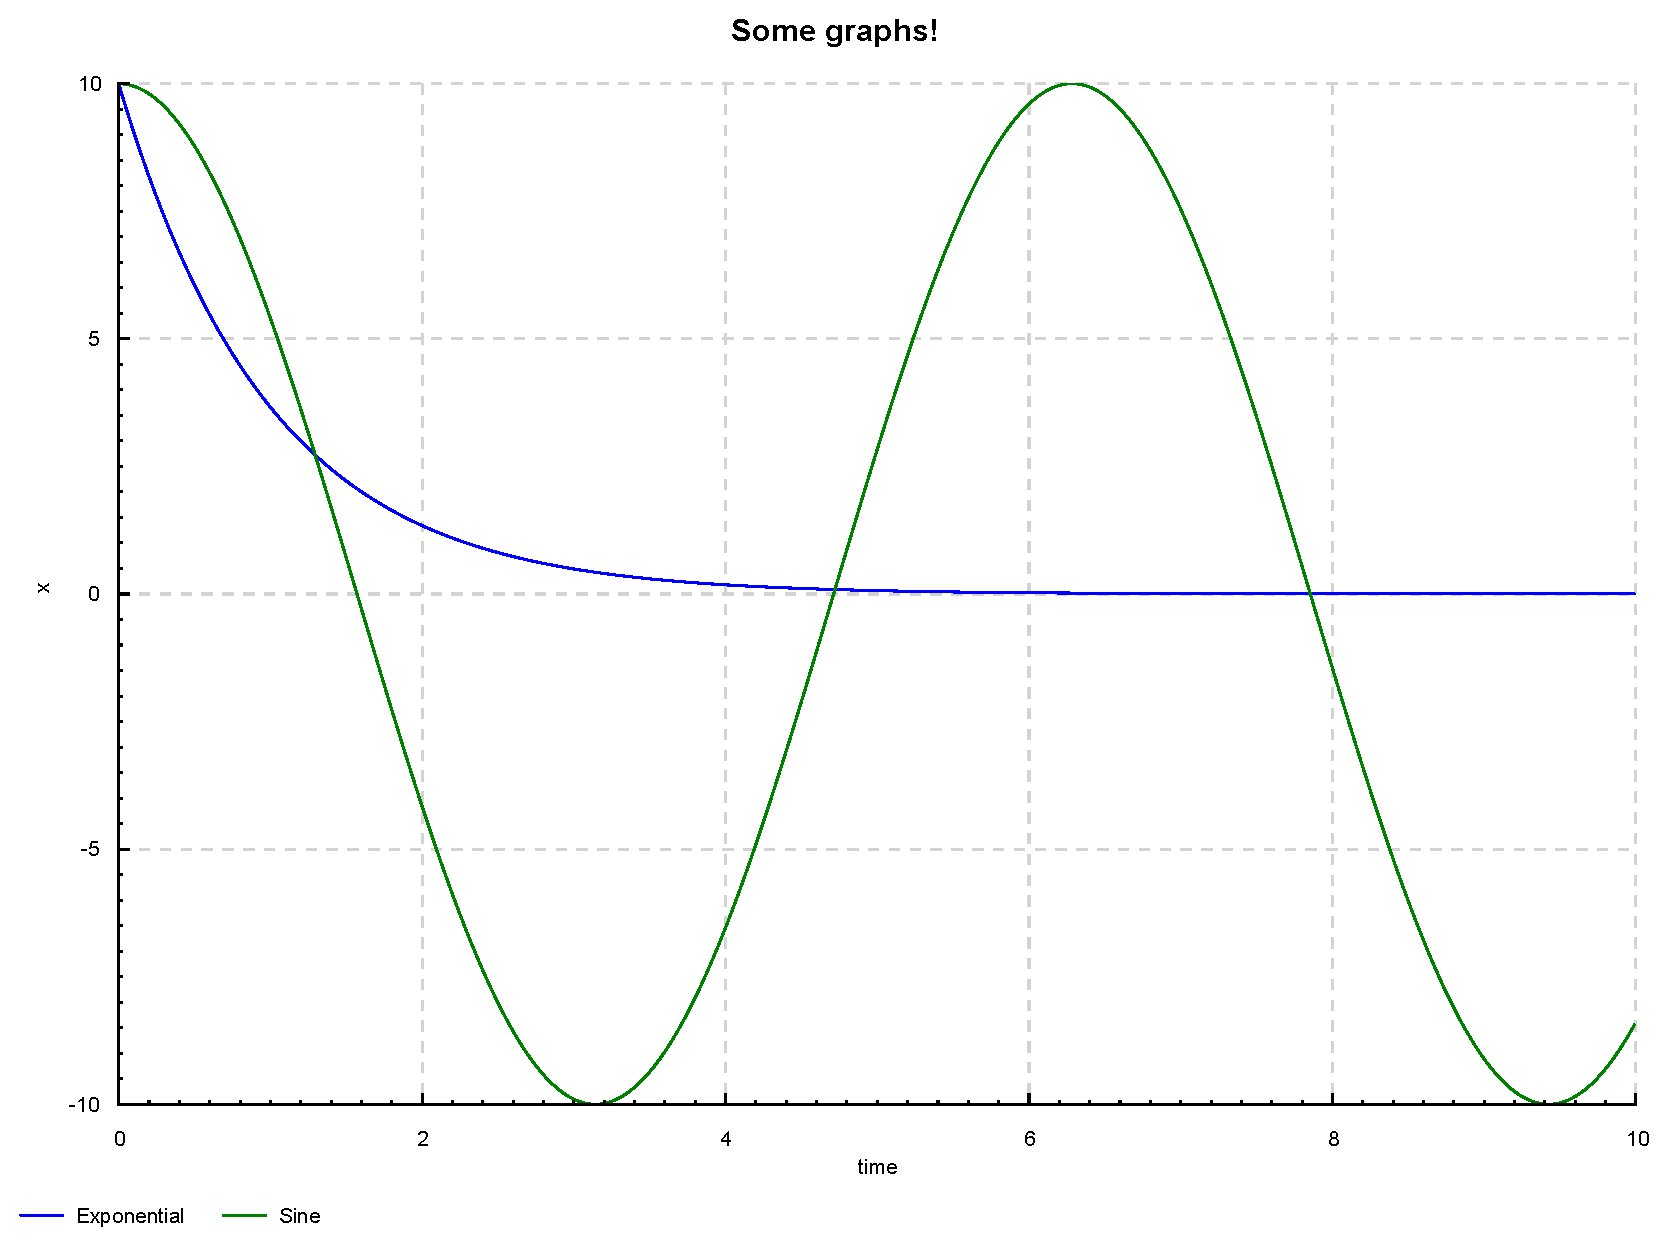
\includegraphics[width=\textwidth]{../haskell/output.pdf}
	\caption{Graphs}
	\label{f:solver_example}
\end{figure}

\begin{align}
\text{Exponential}\sep{}			x(t)' &= -x(t)  \\
\text{Simple harmonic}\sep{}		x(t)'' &= -x(t) \\
\text{Cosine hyperbolic}\sep{}		x(t)' &= \frac{\sqrt{x(t)^{2} - a^{2}}}{a} \\
\text{Simple harmonic}\sep{}		\vecb{x}(t)' &= \begin{bmatrix} 0 & 1 \\ -1 & 0 \\ \end{bmatrix}\vecb{x}(t) \\
\text{Simple forced harmonic}\sep{}	\vecb{x}(t)' &= \begin{bmatrix} 0 & 1 \\ -1 & 0 \\ \end{bmatrix}\vecb{x}(t) + \begin{bmatrix} \sin{(t)} \\ e^{-t} \\ \end{bmatrix}
\end{align}







\section{\clash{}}
\label{s:clash}
\subsection{Designing hardware in a functional way}
\subsection{Mealy machines}